
\chapter{ANALYSIS}
\label{ch:Analysis}

\section{Security}

Now we examine and compare OnioNS' central protocols against our security assumptions and expected threat model.


% Tor circuits work, no global attacker, privacy and anonymity achieved, no crypto breaks
% Tor isn't entirely honest, but the majority is honest
% Eve cannot break Tor in response to OnioNS, Eve cannot guess quorum
% The largest set of agreeing nodes in the Quorum is honest

\subsection{Quorum Selection}

The Quorum nodes have greater attack capabilities than any other class of participants in OnioNS. They have active responsibility over the front of the Pagechain and they must receive, flood, and process new Records from hidden service operators. In our threat model, we assume that an attacker, Eve, already has control of some fixed number $ f_{E} $ of routers in the Tor network, and that her nodes may maliciously collude. We also assume that Eve does does not have motivation to compromise Tor in response to the presence of OnioNS and that she cannot predict future Quorums. It is also impossible to determine which Tor routers are under Eve's control and which are honest in advance, so we examine our Quorum protocols and explore the likelihood of attacks within a probabilistic environment.

The Quorum Derivation protocol selects an $ L_{Q} $-sized subset of routers from the set of Quorum Candidates, and rotates this selection every $ \Delta q $ days. The optimal selection of $ L_{Q} $ and $ \Delta q $ is dependent on both security and performance analysis; our security analysis introduces a lower bound on both $ L_{Q} $ and $ \Delta q $. For the following evaluations, we feel it safe to discard threats that have probabilities at or below $ \frac{1}{2^{128}} \approx 10^{-38.532} $ --- the probability of Eve randomly guessing a 128-bit AES key, a threat that would violate our security assumptions.

Our security analysis assumes that $ L_{Q} $ will be selected from a pool of 5,400 Quorum Candidates --- the number, as of April 2015, of Tor routers with the Fast and Stable flags, whom we assume are all up-to-date Mirrors. Let $ L_{E} $ be the number of Quorum nodes under Eve's control. Then Eve controls the Quorum if the $ L_{E} $ routers become the largest agreeing subset in the Quorum, which can occur if either more than $ \frac{L_{Q} - L_{E}}{2} $ honest Quorum nodes disagree or if $ L_{E} > \frac{L_{Q}}{2} $. The second scenario can be statistically modelled.

Quorum selection is mathematically an $ L_{Q} $-sized random sample taken from an $ N $-sized population without replacement, where the population contains a subset of $ f_{E} $ entities that are considered special. Then the probability that Eve controls $ k $ Tor routers in the Quorum is given by the hypergeometric distribution, whose probability mass function (PMF) is $ \frac{\binom{f_{E}}{k}\binom{N - f_{E}}{L_{Q} - k}}{\binom{N}{L_{Q}}} $. Then the probability that $ L_{E} > \frac{L_{Q}}{2} $ is given by $ \displaystyle\sum_{x=\ceil{\frac{L_{Q}}{2}}}^{L_{Q}} \frac{\binom{f_{E}}{k}\binom{N - f_{E}}{L_{Q} - k}}{\binom{N}{L_{Q}}} $. Odd choices for $ L_{Q} $ prevents the possibility of network disruption when the Quorum is evenly split in terms of the current Page. We examine the probability of Eve's success for increasing amounts of $ f_{E} $ in Figure \ref{chart:quorumMajority}.

\begin{figure}[htbp]
	\centering
	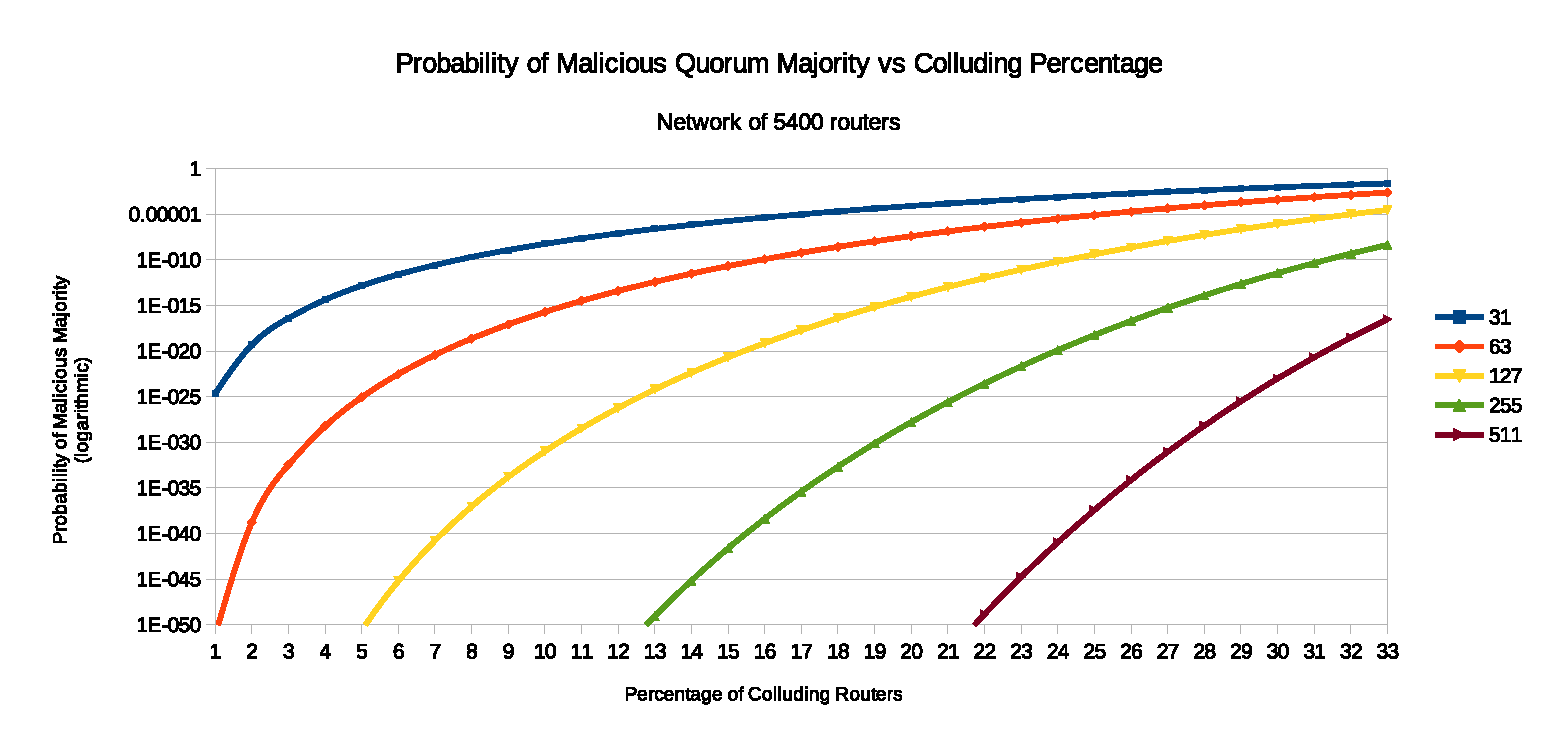
\includegraphics[width=1\textwidth]{analysis/MaliciousQuorumProbability.eps}
	\caption{The probability that Eve controls the majority of the Quorum is given by the PMF of the hypergeometric distribution. We fix $ N $ at 5,400 nodes and graph Eve's success probability as a function of an increasing percentage of Eve-controlled colluding routers. We examine five selections for $ L_{Q} $: 31, 63, 127, 255, and 511. We do not consider percentages beyond 33 percent as 33 percent represents a complete compromise of the Tor network: it is near 100 percent that the three routers selected during circuit construction are under Eve's control, a violation of our security assumptions.}
	\label{chart:quorumMajority}
\end{figure}

Figure \ref{chart:quorumMajority} shows that a choice of $ L_{Q} = 31 $ is suboptimal: the probabilities are above the $ 10^{-38.532} $ threshold for even small levels of collusion. $ L_{Q} = 63 $ likewise fails with approximately two percent collusion, although choices of 127, 255, and 511 fail at levels above approximately 8, 16, and 25 percent, respectively. The figure also suggests that larger Quorums are superior with respect to security. Small Quorums are also less resilient to DDOS attacks at the Quorum in general.

If we assume that Eve controls 10 percent of the Tor network, then we can examine the impact of the longevities of Quorums; over a fixed period of time, slower rotations suggests a lower cumulative chance of selecting any malicious Quorum. If $ w $ is Eve's chance of compromise, then her cumulative chances of compromising any Quorum is given by $ 1 - (1-2)^t $. This gives us a bound estimate on $ \Delta q $. We estimate this over 10 years in Figure \ref{chart:cumulativeProbability}.

\begin{figure}[htbp]
	\centering
	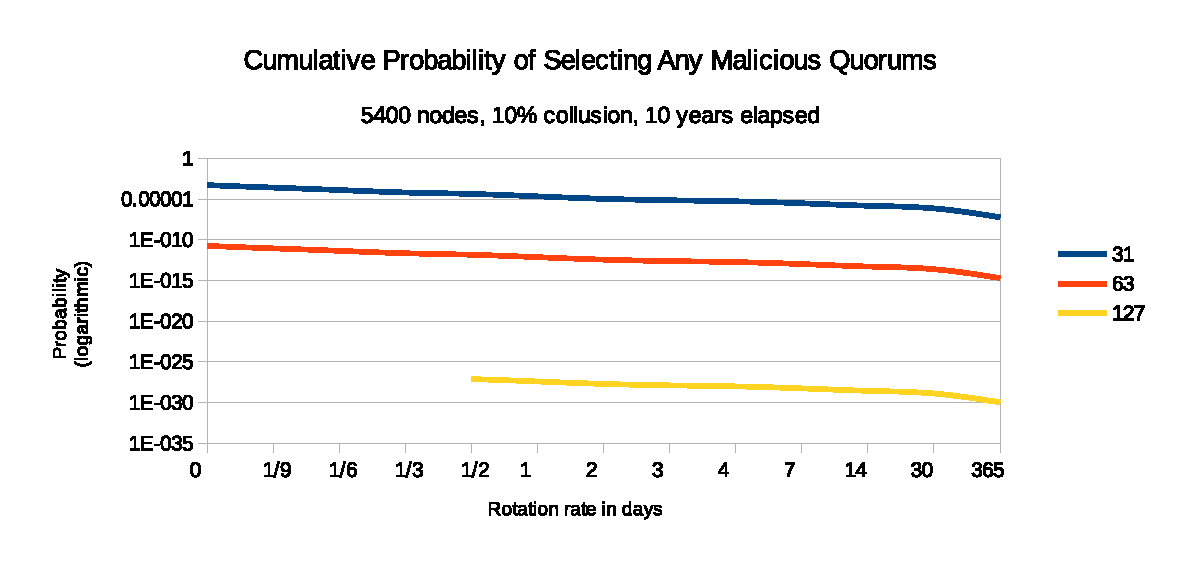
\includegraphics[width=1\textwidth]{analysis/CumulativeMaliciousQuorum.eps}
	\caption{The cumulative probability that Eve controls any Quorum at different rotation rates. We assume 10 percent collusion in a network of 5400 Tor routers, and view across 10 years. We do not graph $ L_{Q} $ values of 255 or 511 as they generate probabilities far below our $ 10^{-38.532} $ threshold; $ L_{Q} = 255 $ and $ L_{Q} = 511 $ produce values less than $ 10^{-58} $ and $ 10^{-134} $, respectively.}
	\label{chart:cumulativeProbability}
\end{figure}

Figure \ref{chart:cumulativeProbability} suggests that while slow rotations (i.e a period of 7 days) generates orders of magnitude less chance than fast rotations, the choice of $ L_{Q} $ is far more significant. Like Figure \ref{chart:quorumMajority}, it also shows that $ L_{Q} = 31 $ and $ L_{Q} = 61 $ are relatively poor choices.

If a selected Quorum is malicious, fast rotation rates will minimize the duration of any disruptions, as shown in Figure \ref{chart:quorumLongevity}. This figure suggests that fast rotations are optimal in that respect, a contradiction to Figure \ref{chart:quorumMajority}. However, given the very low statistical likelihood of selecting a malicious Quorum, we consider this a minor contribution to the decision.

\begin{figure}[htbp]
	\centering
	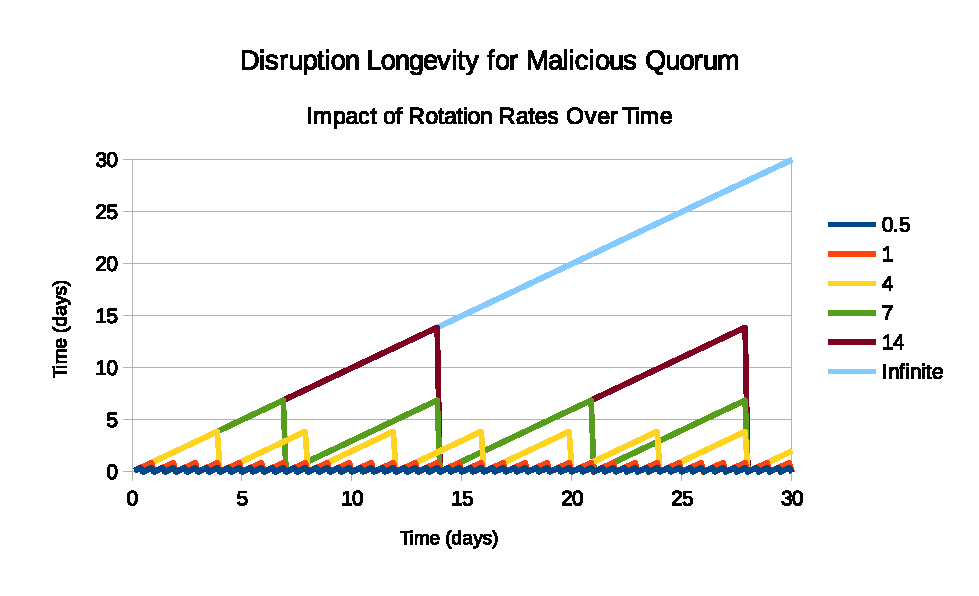
\includegraphics[width=1\textwidth]{analysis/MaliciousLongevityRotations.eps}
	\caption{The duration of malicious Quorums as a function of different rotation rates. Quorums that have very short livetimes (and are thus rotated quickly) minimize the duration of any malicious activity.}
	\label{chart:quorumLongevity}
\end{figure}

Although a malicious Quorum would have the capabilities to deploy a variety of attacks on the network, the proper selections of $ L_{Q} \geq 127 $ and $ \Delta q \geq 1 $ reduces the likelihood of this occurring to near-zero probabilities. We consider this a stronger solution than introducing countermeasures to those attacks. Based on our security analysis, we suggest $ L_{Q} \geq 127 $ and $ \Delta q \geq 1 $.

\newpage

\subsection{Entropy of Tor Consensus Documents}
\label{sec:docEntropy}

We use Tor's consensus documents as a sources of entropy agreed upon by all parties, however we have not yet demonstrated that the network status contains enough entropy to provide reasonable assurance that Eve cannot guess the next Quorum in advance. If Eve could predict future Quorums, Eve can subvert the Quorum Derivation protocol in a variety of attack vectors. However, this would fail our security assumption against adaptive compromise in the presence of OnioNS. Rather than introducing defences against these attack vectors, we nevertheless believe that ensuring sufficient entropy in the consensus documents is a superior defence.

%	\item \textbf{dir-source:} The authority's nickname, fingerprint, IP address, onion routing port, and directory port.
%	\item \textbf{contact:} Optional contact information for the authority operator.
%	\item \textbf{vote-digest:} The hash of the authority's status vote document.
%	
%	\item \textbf{r:} The router's nickname, fingerprint, time of last restart, IP address, onion routing port, and directory port.
%	\item \textbf{m:} The SHA-256 hash of the router's microdescriptor. This also includes its entries in the \emph{cached-microdescs} document (discussed below).
%	\item \textbf{s:} A list of the router's status flags, as given by the directory authorities. Common examples include Running, Valid, Fast, Guard, Stable, and Exit.
%	\item \textbf{v:} The version of the Tor software that the router is running, as reported by the router.
%	\item \textbf{w:} The estimated bandwidth that this router is capable of. This value is determined by speed tests from bandwidth authorities, who are a subset of the directory authorities.

In section \ref{sec:ConsensusDocs} we detailed the significant contents of the three consensus documents relevant to OnioNS, \emph{cached-certs}, \emph{cached-microdesc-consensus}, and \emph{cached-microdescs}. As we stated in section \ref{sec:Protocols}, the Quorum Derivation protocol only utilizes the \emph{cached-certs} and \emph{cached-microdesc-consensus} documents for reasons we discuss below.

\subsubsection{cached-certs}

The \emph{cached-certs} document contains long-term directory identity keys and medium-term signing keys. While Eve cannot predict the public half of new signing keys in advance, the keys rotate every 3-12 months\cite{TorDirSpec} so \emph{cached-certs} is not a timely source of entropy. Nevertheless, if an attacker can predict the network status described in \emph{cached-microdesc-consensus}, the rotation timeline of the signing keys in \emph{cached-certs} places an absolute upper-bound on the duration of Quorum predictability.

\subsubsection{cached-microdesc-consensus}

The \emph{cached-microdesc-consensus} document describes the network status and is our main source of entropy. In the header, the  \emph{vote-digest} header is the hash of a directory authority's status vote. Each directory operates independently and there are nine directory authorities, so we consider this value unpredictable. Router descriptors follow the header in the body of the document. 

The $ r $ field in a router's descriptor contains routing information and time of last restart. Tor routers have no guarantee of availability and routers may restart for a variety of reasons. As of April 2015 Tor's network consists of approximately 7,000 routers \cite{TorMetrics} and assuming that a given router restarts every 60 days, statistically the number of unpredictable $ \emph{r} $ fields each day is given by $ \frac{7000}{60} \approx 116.66 $. Tor displays the restart time down to the second, so each restart adds approximately six bytes of entropy, for an estimated total of $ \frac{7000 * 6}{60} = 700 $ bytes of short-term entropy from the $ r $ field.

%The $ s $ field contains a list of flags given to the router by the directory authorities according to qualification rules. $ s $ is thus predictable if an attacker can monitor the descriptor

The $ v $ field describes the version of Tor that the router is running. Although the versions of Tor are publicly known and the official and unofficial Linux repositories are publicly accessible, Eve cannot predict when an administrator will upgrade their router to the next available Tor version. Although new versions of Tor are not frequently released and routers are upgraded infrequently as shown in Figure \ref{fig:TorVersions}, the $ v $ field still introduces a degree of medium-term entropy into the document.

\begin{figure}[htbp]
	\centering
	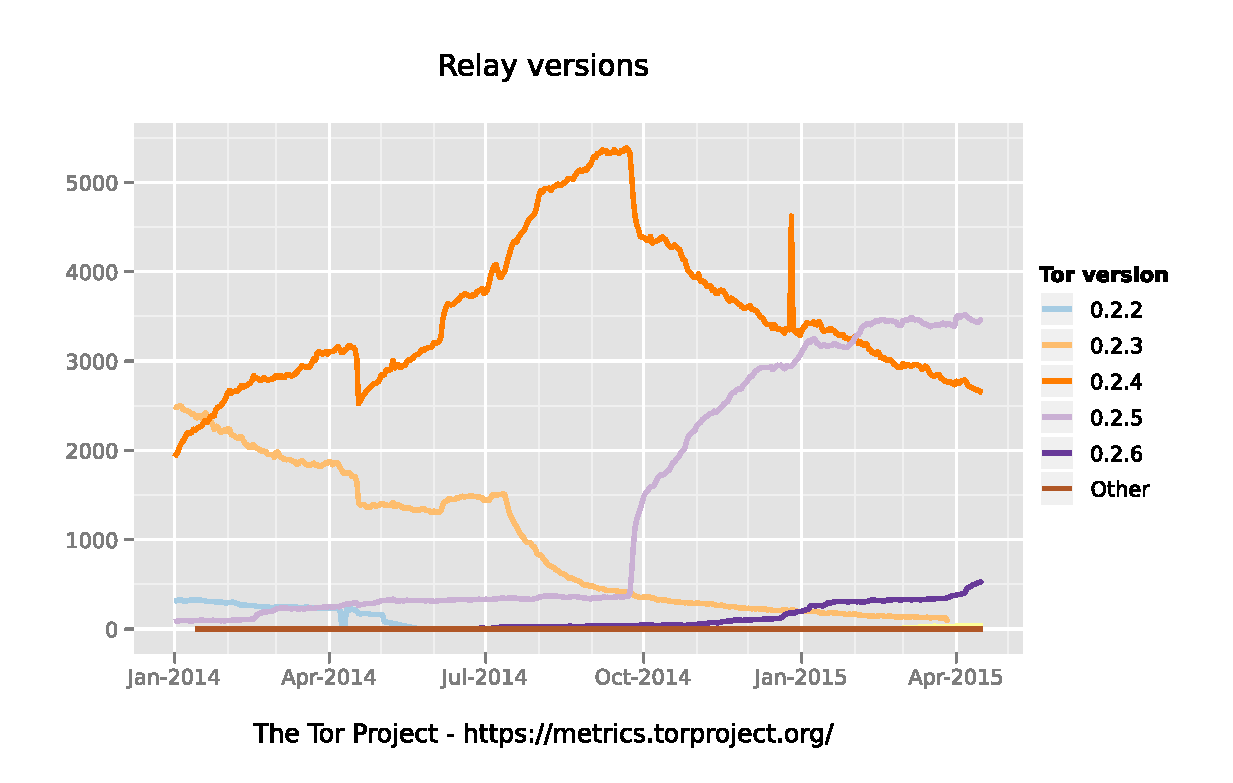
\includegraphics[width=0.95\textwidth]{images/Tor/versions_2014-01_2015-04.eps}
	\caption{The versions of Tor software between January 2014 and April 2015.\cite{TorMetrics}}
	\label{fig:TorVersions}
\end{figure}

The $ w $ field contains the router's estimated bandwidth capacity as calculated by bandwidth authorities. Clients use this field during circuit construction; routers with a higher bandwidth capacity relative to the rest of the network have a higher probability of being included in a circuit. Although it is likely that a given router will have similar bandwidth measurements between consecutive consensus documents, Eve cannot predict the exact performance of a router from the perspective of the bandwidth authority. Eve's capacity to predict the performance of all routers falls outside of Tor's and OnioNS' security assumptions; Eve must therefore be a global attacker who would be capable of compromising the Tor network as a whole anyway.

We note that significant amounts of additional entropy could be trivially added into \emph{cached-microdesc-consensus} if each router added a single random byte to their descriptor or if the directory authorities each contributed entropy.

\subsubsection{cached-microdescs}

Although we did not detail it in section \cite{TorDirSpec}, in practice Tor places client-side timestamps inside \emph{cached-microdescs}. These timestamps would significantly divide the network, causing \emph{cached-microdescs} to be ill-suited for inclusion in the Quorum Derivation protocol. Although \emph{cached-microdescs} contains long-term router keys and the fingerprints of routers in the same family which would both serve as a source of long-term entropy, \emph{cached-microdesc-consensus} contains the SHA-256 hashes of the router descriptor. We therefore do not include it when hashing the documents in the Quorum Derivation protocol.

\subsubsection{General Analysis}

The Quorum Derivation protocol describes initializing the Mersenne Twister with a 384-bit seed. If we assume that Eve desires that the Quorum Derivation protocol produce a Quorum pleasing to Eve (such as including her malicious routers in the Quorum or rejecting specific honest routers from the Quorum) then Eve can find $ k $ seeds that generates a desirable scrambled list in $ 2^{192} $ operations on average, or $ 2^{384} $ operations in the worst case. The chance of any of those seeds being selected is $ \frac{2^{384}}{k} $. 

If we also assume that Eve can predict some fraction $ f \in {(0, 1)} $ of the contents of the consensus documents, then Eve may attempt to manipulate her router's descriptors such that the Quorum Derivation protocol produces one of the $ k $ hashes. SHA-384's strong resistance to preimage and second preimage attacks requires $ 2^{192} $ operations on average for Eve to find one of the $ k $ hashes. This difficulty is compounded by the limited combinatorics within the set of valid router descriptors. The number of operations involved in this attack vector is significantly more than the operations involved in breaking AES, so we disregard the possibility of manipulating the Quorum Derivation protocol in this way. We do not consider the possibility of Eve controlling the entire consensus document, this would severely compromise the integrity of the Tor network and thus violates our security assumptions.

\subsection{Sybil Attacks}

Eve may also attempt to increase her probability of including her malicious nodes in the Quorum via Sybil attacks. We offer no defence against this type of attack, although Tor does. The attack is difficult to carry out in practice due to the slow build of trust within the Tor network. Directory authorities would give Eve's nodes the Fast and Stable flags after weeks of continual uptime and a history of reliability. For large-scale Sybil attacks, this introduces a significant time and financial cost to Eve. We also note that choices of $ L_{Q} $ and $ \Delta q $ also offer significant statistical defences against Sybil attacks, as illustrated in Figures  \ref{chart:quorumMajority} and \ref{chart:cumulativeProbability}, shown above.

\subsection{Hidden Service Spoofing}

OnioNS does not require a hidden service operator to reveal any personally-identifiable information. Hidden services are only known by their public key and domain names, and we assume that the hidden service is authentic. We have also observed spoofed hidden services in the wild, suggesting that this problem already exists in Tor's environment. We do not introduce a reputation system or distributed verification system, and note that it is difficult if not impossible to construct a reliable defence against hidden service spoofing attacks due to their anonymous nature. 

One possible solution, although it severely compromises anonymity, is to register a hidden service with an SSL Certificate Authority and apply an SSL certificate to the server. In this way, TLS communication provides an authenticity check against the hidden service, although TLS also sets up a redundant encryption layer that may decrease performance. However, in practice this solution is very rarely seen; out of approximately 25,000 hidden services,\cite{TorMetrics}\cite{kadianakis2015extrapolating} to date only three hidden services have browser-trusted SSL certificates: Blockchain.info at https://blockchainbdgpzk.onion, Facebook at https://facebookcorewwwi.onion, and The Intercept's SecureDrop instance at https://y6xjgkgwj47us5ca.onion. In future work we may study the security implications of signing the .onion address or the .tor OnioNS domain name. Due to their severe privacy concerns and the security controversy surrounding the centralized CA Chain of Trust, generally speaking we do not recommend the application of SSL certificates to Tor hidden services. 

\subsection{Outsourcing Record Proof-of-Work}

%Scrypt introduces a cost and its memory demands increases the difficulty of custom hardware and massively-parallel attacks, effectively limiting adversaries to the same hardware as legitimate users.

The Record Generation protocol can safely take place within an offline machine under the operator's control. We designed the Record Generation protocol with the objective of requiring the hidden service operator to also perform the scrypt proof-of-work. However, our protocol does not entirely prevent the operator from outsourcing the computation to secondary resource in all cases.

Let Bob be the hidden service operator, and let Craig be a secondary computational resource. We assume that Craig does not have Bob's private key. Then,

\begin{enumerate}
	\item Bob creates an initial Record $ R $ and completes the \emph{type}, \emph{nameList}, \emph{contact}, \emph{timestamp}, and \emph{consensusHash} fields.
	\item Bob sends $ R $ to Craig.
	\item Let $ \mathit{central} $ be $\mathit{type} \concat \mathit{nameList} \concat \mathit{contact} \concat \mathit{timestamp} \concat \mathit{consensusHash} \concat \mathit{nonce} $.
	\item Craig generates a random integer $ K $ and then for each iteration $ j $ from 0 to $ K $,
		\begin{enumerate}
			\item Craig increments \emph{nonce}.
			\item Craig sets \emph{PoW} as $ \mathrm{PoW}(\mathit{central}) $.
			\item Craig saves the new $ R $ as $ C_{j} $.
		\end{enumerate}
	\item Craig sends all $ C_{0 \le j \le K} $ to Bob.
	\item For each Record $ C_{0 \le j \le K} $ Bob computes
		\begin{enumerate}
			\item Bob sets \emph{pubHSKey} to his public RSA key.
			\item Bob sets \emph{recordSig} to $ S_{d}(m, r) $ where $ m = \mathit{central} \concat \mathit{pow} $ and $ r $ is Bob's private RSA key.
			\item Bob has found a valid record if $ H(\mathit{central} \concat \mathit{pow} \concat \mathit{recordSig}) \leq 2^{\mathit{difficulty} * \mathit{count}} $
		\end{enumerate}
\end{enumerate}

% todo: calculate chances of Craig computing a correct record

Our protocol ensures that Craig must always compute more scrypt iterations than necessary; Craig cannot generate \emph{recordSig} and thus cannot compute if the hash is below the threshold. Moreover, the scrypt work incurs a cost onto Craig that must be compensated financially by Bob. Thus the Record Generation protocol places a lower bound on the cost paid by Bob.

%\subsection{False Negatives Claims}
%
%OnionNS records are self-signed and include the hidden service's public key, so anyone --- particularly the client --- can confirm the authenticity (relative to the authenticity of the public key) and integrity of any record. This does not entirely prevent Sybil attacks, but this is a very hard problem to address in a distributed environment without the confirmation from a central authority. However, the proof-of-work component makes record spoofing a costly endeavour, but it is not impossible to a well-resourced attacker with sufficient access to high-end general-purpose hardware.
%
%Hidden service .onion addresses will continue to have an extremely high chance of being securely unique as long the key-space is sufficiently large to avoid hash collisions.
%
%As we have stated earlier, falsely claiming a negative on the existence of a record is a problem overlooked in other domain name systems. One of the primary challenges with this approach is that the space of possible names so vast that attempting to enumerate and digitally sign all names that are not taken is highly impractical. Without a solution, this weakness can degenerate into a denial-of-service attack if the DNS resolver is malicious towards the client. Our counter-measure is the highly compact hashtable bitset with a Merkle tree for collisions. We set the size of the hashtable such that the number of collisions is statistically very small, allowing an efficient lookup in $ \mathcal{O}(1) $ time on average with minimal data transferred to the client.

\subsection{DNS Leakage}

Human mistakes can also compromise user privacy. One such security threat is the accidental leakage of .tor lookups over the Internet DNS. This vulnerability is not limited to OnioNS and applies to any alternative DNS; users may mistakenly attempt lookups over the traditional Internet DNS. Mohaisen and Thomas observed .onion lookups on root DNS servers at a frequency that corresponded to external global events, highlighting the human factor in those leakages.\cite{thomasmeasuring} For OnioNS, this may occur if their client software was not properly configured, if their browser was not properly configured to or could not communicate with Tor, or for other reasons. We offer no defence against this attack vector and note that any defence against it would need to introduce lookup whitelists or blacklists into common browsers such as Chrome, Firefox, and Internet Explorer to prevent them from attempting lookups for pseudo-TLDs.

%\section{Reliability}

%\subsubsection{Flooding}

%\emph{What happens if Quorum nodes are unavailable? How is their unavailability secured for future reference? What are the implications of a Quorum node withholding or forging a Record before flooding their Snapshot out? Can a single node mislead the rest of the Quorum?}

%Although this approach does not entirely thwart Sybil attack, this attack vector is difficulty to impossible to counter in a privacy-enhanced environment, and trading anonymity for defence is highly undesirable.

%\emph{Tor nodes provide no guarantee of availability. What are the implications of Quorum nodes or Mirrors suddenly disappearing? How can data be lost? What if a Quorum node is offline temporarily during active duty, will it catch up?}

%  on Unreliable Hosts

%Tor nodes have no reliability guarantee and may disappear from the network momentarily or permanently at any time. Old \emph{quorums} may disappear from the network without consequence of data loss, as their data is cloned by current \emph{mirrors}. So long as the \emph{quorum} nodes remain up for the $ \Delta i $ days that they are active, the system will suffer no loss of functionality. Nodes that become temporarily unavailable will have out-of-sync \emph{pages} and will have to fetch recent records from other \emph{quorum} nodes in the time of their absence.

\section{Objectives Assessment}

OnioNS achieves all of our original requirements:

\begin{enumerate}
	\item \textbf{The system must support anonymous registrations} --- OnioNS Records do not contain any personal or location information. The PGP key field is optional and may be provided if the hidden service operator wishes to allow others to contact him. However, the operator may be using an email address and a Web of Trust disassociated from his real identity, in which case no identifiable information is exposed.
	\item \textbf{The system must support privacy-enhanced lookups} --- OnioNS performs Domain and Onion Queries through Tor circuits, and under our original assumption that circuits provide strong guarentees of client privacy and anonymity, resolvers cannot sufficiently distinguish users to track their lookups.
	\item \textbf{Clients must be able to authenticate registrations} --- OnioNS Records are self-signed, enabling Tor clients to verify the digital signature on the domain names and check the public key against the server's key during the hidden service protocol. This ensures that the association has not been modified in transit and that the domain name is authentic relative to the authenticity of the destination server.
	\item \textbf{Domain names must be provably or have a near-certain chance of being unique} --- Tor hidden services .onion addresses are cryptographically generated with a key-space of $ 58 ^ {16} \approx 2 ^ {93.727695922} $ and domain names within OnioNS are provably unique by anyone holding a complete copy of the Pagechain.
	\item \textbf{The system must be distributed} --- The responsibilities of OnioNS are spread out across many nodes in the Tor network, decreasing the load and attack potential for any single node. The Pagechain is likewise distributed and locally-checked by all Mirrors, and although its head is managed by the Quorum, these authoritative nodes have temporary lifetimes and are randomly selected. Moreover, Quorum nodes do not answer queries, so they have limited power.
	\item \textbf{The system must be simple and relatively easy to use} --- Domain Queries are automatically resolved and require no input by the user. From the user's perspective, they are taken directly from a meaningful domain name to a hidden service. Users no longer have to use unwieldy .onion addresses or review third-party directories, OnioNS introduces memorability to hidden service domains.
	\item \textbf{The system must be backwards compatible with existing protocols} --- OnioNS does not require any changes to the hidden service protocol and existing .onion addresses remain fully functional. Our only significant change to Tor's infrastructure is the mechanism for distributing hashes for the Quorum Qualification protocol, but our initial technique for using the Contact field minimizes any impact. We also hook into Tor's TLD checks, but this change is very minor. Our reference implementation is provided as a software package separate from Tor per the Unix convention.
\end{enumerate}

Finally, we meet our optional performance objectives:

\begin{enumerate}
	\item \textbf{The system should not require clients to download the entire database} --- Only Mirrors hold the Pagechain, and clients do not need to obtain it themselves to issue a Domain Query. Therefore clients rely on their existing and well-established trust of Tor routers when resolving domain names. However, clients may optionally obtain the Pagechain and post Domain Queries to localhost for greater privacy and security guarantees.
	\item \textbf{The system should not introduce significant burdens to the clients} --- Record verification should occur in sub-second constant time in most environments, and Ed25519 achieves very fast signature confirmation so verifying Page signatures at level 1+ takes trivial time. However, clients also verify the Record's proof-of-work, so for some scrypt parameters the client may spend non-trivial CPU time and RAM usage confirming the one scrypt iteration required to check. We must therefore choose our parameters carefully to reduce this burden especially on low-end hardware.
	\item \textbf{The system should have low latency} --- Domain Queries without any packet delays over Tor low-latency circuits. Its exact performance is largely dependent on circuit speed and the client's verification speed.
\end{enumerate}

We therefore believe that we have squared Zooko's Triangle; OnioNS is distributed, enables hidden service operators to select human-meaningful domain names, and domain names are guaranteed unique by all participants.
